% !TEX root = main.tex

\jparagraph{Encoding Name-Passing into Process-Passing.}

Our main contribution is 
an encoding of \HOp into \HO (\secref{subsec:HOpi_to_HO}).  
Since \HO lacks 
both name-passing and recursion, this encoding involves two key challenges:
\begin{enumerate}[a.]
\item In known (typed) 
encodings of name-passing into process-passing~\cite{SaWabook} %are limited: % in that 
%they come with restrictions on name usages;  
%they 
%work for %name-passing 
%calculi 
%with \emph{capability types} 
%in which 
only the output capability of names can be sent---a received name cannot be used in later inputs.
This is far too limiting in \HOp, where 
 session names %denoting arbitrary protocols 
 may be passed around (\emph{delegation})
and types describe interaction  \emph{structures}, rather than ``loose'' name capabilities. % at a given time.

\begin{figure}[t]
\centering
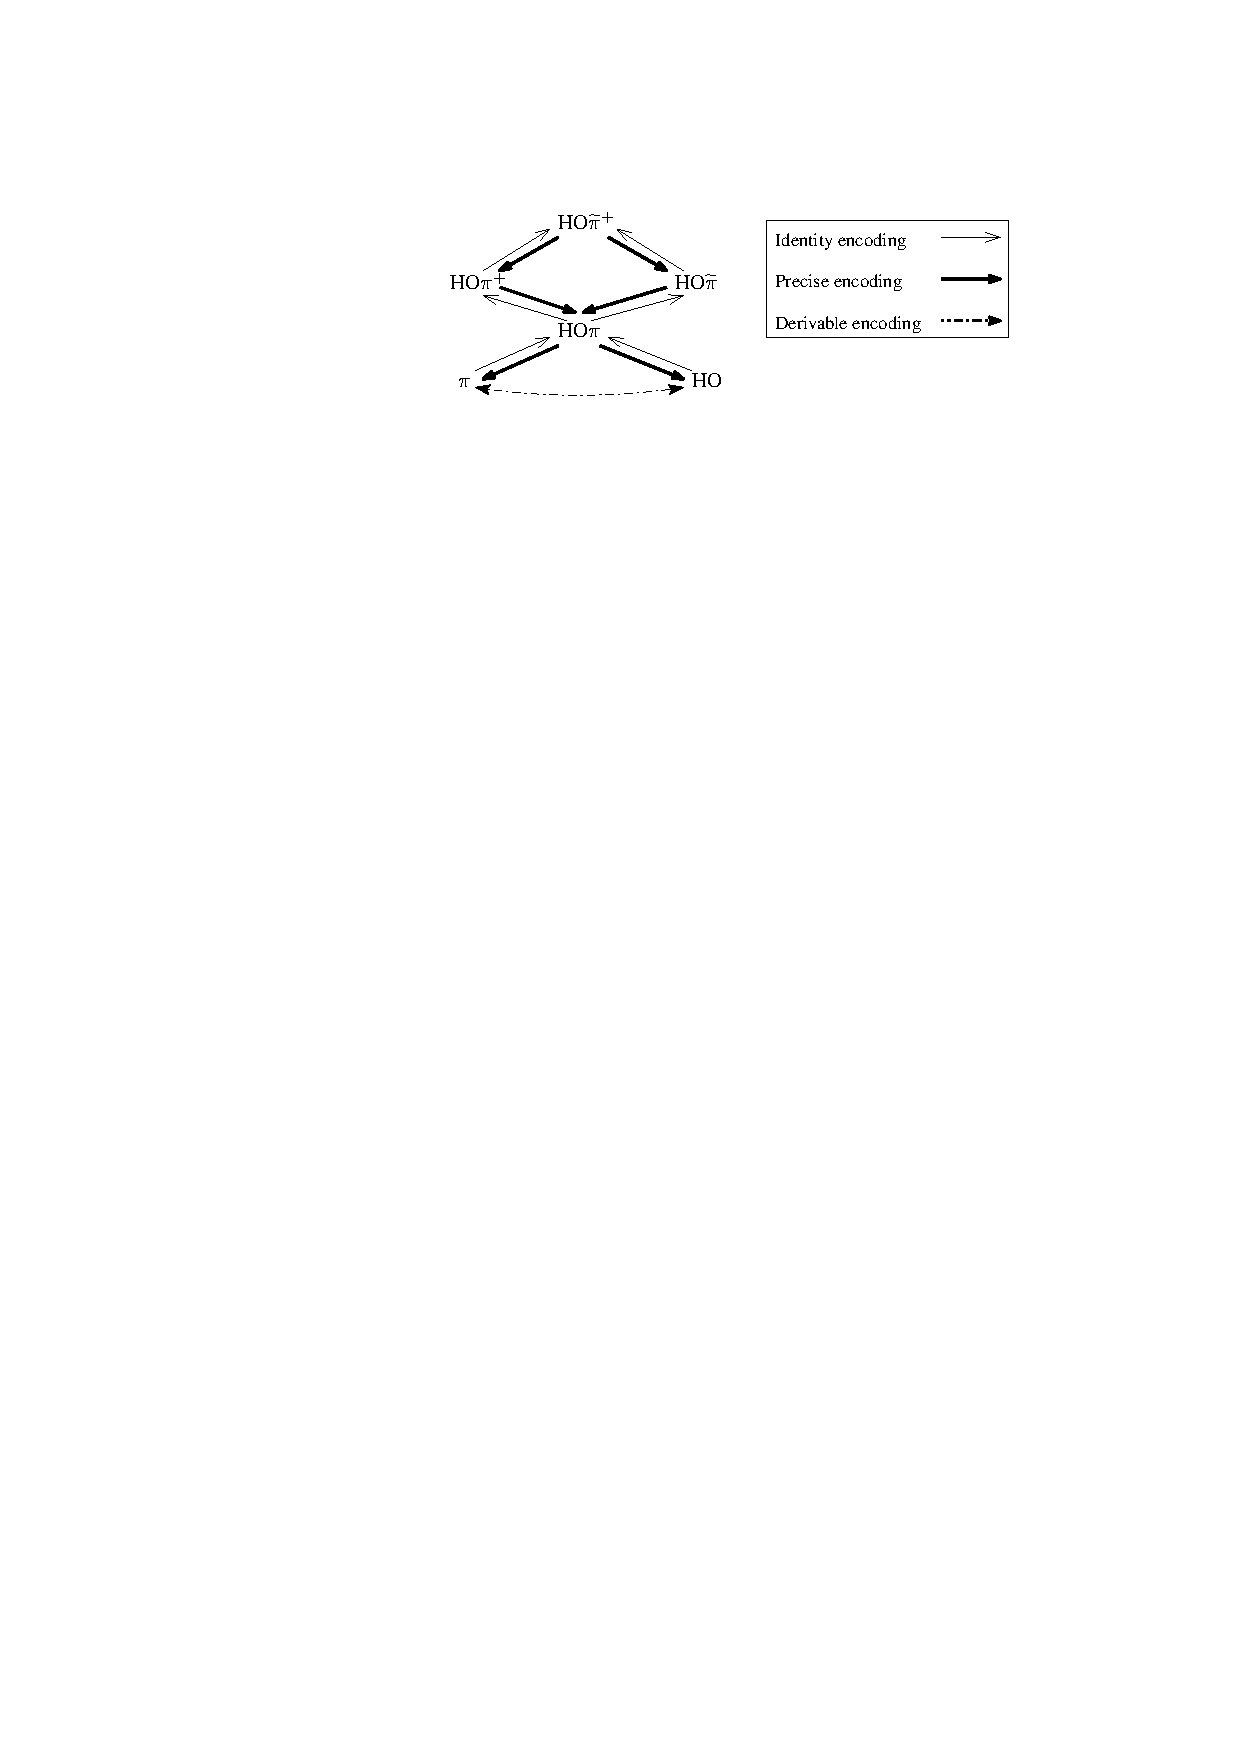
\includegraphics[scale=1]{diag.pdf}
%\vspace{1mm}
	\caption{Encodability in Higher-Order Sessions. 
	Precise encodings are defined in \defref{def:goodenc}.
	\label{fig:express}}
\Hlinefig
\end{figure}

\item %As mentioned above, recursion % and replication)
%can be encoded in untyped higher-order calculi using process duplication. Unfortunately, this kind of encodings 
Known encodings of recursion in untyped higher-order calculi
do not carry over to session typed calculi such as \HOp,
because linear abstractions cannot be copied/duplicated. Hence, the discipline of session types  limits 
the possibilities for representing infinite behaviors---even simple forms, such as input-guarded replication.
\end{enumerate}




%MOTIVATION FIRST ENCODING (). \emph{Still to highlight: recursive type required, no recursion, small example.

%--- 
\noi
%We illustrate our approach. % to these challenges.
Our encoding overcomes these two obstacles. 
Concerning (a), %we illustrate the essence of 
to encode name passing into \HO, 
%to encode name output, 
we ``pack''
the name to be sent into a suitable abstraction; 
upon reception, the receiver must ``unpack'' this object following a precise protocol on a fresh  session:
%More precisely, our encoding \jpc{of name passing} in \HO is given as:
\begin{center}
\begin{tabular}{rcll}
  $\map{\bout{a}{b} P}$	&$=$&	$\bout{a}{ \abs{z}{\,\binp{z}{x} (\appl{x}{b})} } \map{P}$ \\
  $\map{\binp{a}{x} Q}$	&$=$&	$\binp{a}{y} \newsp{s}{\appl{y}{s} \Par \bout{\dual{s}}{\abs{x}{\map{Q}}} \inact}$
\end{tabular}
\end{center}
%and as a homomorphism for the other operators.
Above, 
%where
$a,b$ are names and $s$ and $\dual{s}$ are 
linear session names (\emph{endpoints}).
%$\lambda x.P$ is a name abstraction of $P$; $\appl{x}{a}$ is a name application; 
Processes $\bout{a}{V} P$ and 
$\binp{a}{x} P$ denote output and input at~$a$;   
abstractions and applications are denoted
$\lambda x.P$ and $(\lambda x.P)a$; %, respectively;
$\newsp{s}P$ and $\inact$ represent hiding and inaction. %, respectively.
%Intuitively, the output of a name $b$ along name $a$ is encoded by
%the output of an abstraction containing $b$; the input of a name is encoded 
%by the input of an abstraction
Thus, following a communication on $a$, %our encoding features 
a (deterministic) reduction between  
$s$ and $\dual{s}$ guarantees that name $b$ is properly unpacked by means of abstraction passing
and appropriate applications.



Concerning (b), encoding a recursive process  is \NY{also} challenging for 
%the linearity of endpoints in $P$ must be preserved.
%The encoding of a recursive process $\recp{X}{P}$  is delicate, for it 
it must preserve the linearity of session endpoints. 
Given $\recp{X}{P}$, 
we encode the recursion body $P$ as a name abstraction
in which free names of $P$ are converted into name variables.
%The encoding keeps track of these free names.
The resulting higher-order value is embedded in an input-guarded 
``duplicator'' process~\cite{ThomsenB:plachoasgcfhop}.
Each occurrence of the recursion variable $X$ is then encoded 
in such a way that it
simulates recursion unfolding by 
invoking the duplicator in a by-need fashion.
That is, upon reception, the abstraction representing the 
recursion body $P$
is duplicated: 
one copy is used to reconstitute the original recursion body $P$ (through
the application of the free names of $P$); 
another copy is used to re-invoke the duplicator when needed. 
Interestingly, for this encoding strategy to work 
we require non-tail recursive session types; to this end, 
we apply recent advances on the theory of duality for session types~\cite{TGC14,DBLP:journals/corr/abs-1202-2086}.

%To this end, we
%first record a mapping from recursive variable $X$ to process variable $z_X$.
%Then, we encode the recursion body $P$ as a name abstraction
%in which free names of $P$ are converted into name variables, using \defref{d:auxmap}.
%(Notice that $P$ is first encoded into \HO and then transformed using mapping
%$\auxmapp{\cdot}{{}}{\sigma}$.)
%Subsequently, this higher-order value is embedded in an input-guarded 
%``duplicator'' process~\cite{ThomsenB:plachoasgcfhop}. Finally, we define the encoding of $X$ 
%in such a way that it
%simulates recursion unfolding by 
%invoking the duplicator in a by-need fashion.
%That is, upon reception, the \HO abstraction which encodes  the 
%recursion body $P$
%%containing $\auxmapp{P}{{}}{\sigma}$ 
%is duplicated: 
%one copy is used to reconstitute the original recursion body $P$ (through
%the application of $\fn{P}$); another copy is used to re-invoke
%the duplicator when needed. 
%
%We encode recursion with non-tail recursive session types; for this 
%we apply recent advances on the theory of session duality~\cite{TGC14,DBLP:journals/corr/abs-1202-2086}.

\jparagraph{Precise Encodings}
Before closing this section, we find it instructive to discuss the notion of encoding 
upon which our 
encodability results stand.
Building upon established notions for (untyped) processes (e.g.,~\cite{DBLP:journals/iandc/Gorla10}), 
we define a notion of \emph{precise encoding} (\secref{s:expr}) that, as motivated earlier,  
requires the translation of both process and types, and 
admits only process mappings that preserve session types
\emph{and} are fully abstract. Thus, our encodings 
exhibit   strong behavioral correspondences, and 
 relate source and target processes with  
proper communication structures (as described by session types).
%Moreover, the notion of encoding includes full abstraction as encodability criteria.
We argue that these requirements make our developments more challenging.
In particular, requiring type preservation rules out encoding strategies only plausible for untyped processes.
To illustrate this point,
consider the  following encoding of %$\sessp$ 
name-passing 
into $\HO$:\footnote{This alternative  encoding was suggested by an anonymous reviewer of a previous version of this paper.} %defined as
\begin{center}
\begin{tabular}{rcll}
  $\umap{\bout{a}{b} P}$	&$=$&	$\binp{a}{x}( \appl{x}{b} \Par \umap{P})$ \\
  $\umap{\binp{a}{x} Q}$	&$=$&	$\bout{a}{\abs{x}{\umap{Q}}} \inact$
\end{tabular}
\end{center}
%and as a homomorphism for the other operators.
Intuitively, 
rather than sending a package with name $b$, 
this encoding sends the continuation of the input. This entails  a 
``role inversion'': outputs are translated into inputs, and inputs are translated into outputs. 
Although perfectly reasonable in an  {untyped setting}, the encoding $\umap{\cdot}$  
%is far from desirable in a session typed setting: 
is \emph{not type preserving}: 
since 
individual  prefixes represent actions in a structured communication sequence (abstracted by session types)
the role inversion defined by $\umap{\cdot}$ would alter the meaning of session protocols in the source language.



